\section{Anhang}

\subsection{Teil I: Kalibrierung}

\subsubsection{Fixpunktkalibration an der Wassertripelpunktzelle}

\begin{figure}[H]
	\centering
	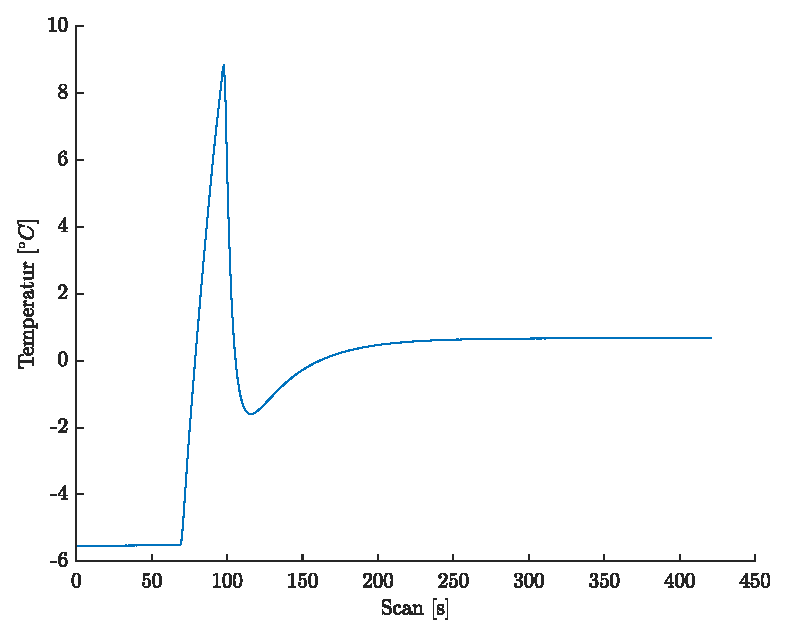
\includegraphics[height=0.2\textheight]{../MLAB/Fixpunktkalibration.eps}
	\caption[Temperaturverlauf des Pt100 Temperatursensors mittels Wassertripelpunktzelle]{ Temperaturverlauf des Pt100 Temperatursensors mittels Wassertripelpunktzelle im Metallblockkalibrator.}
	\label{fig:Fixpunkt}
\end{figure}

\subsection{Teil III: Wärmebildkamera}

Aufgenommene Bilder des Versuchsstandes und Bilder der Wärmebildkamera. 

\begin{figure}[H]
		\centering
		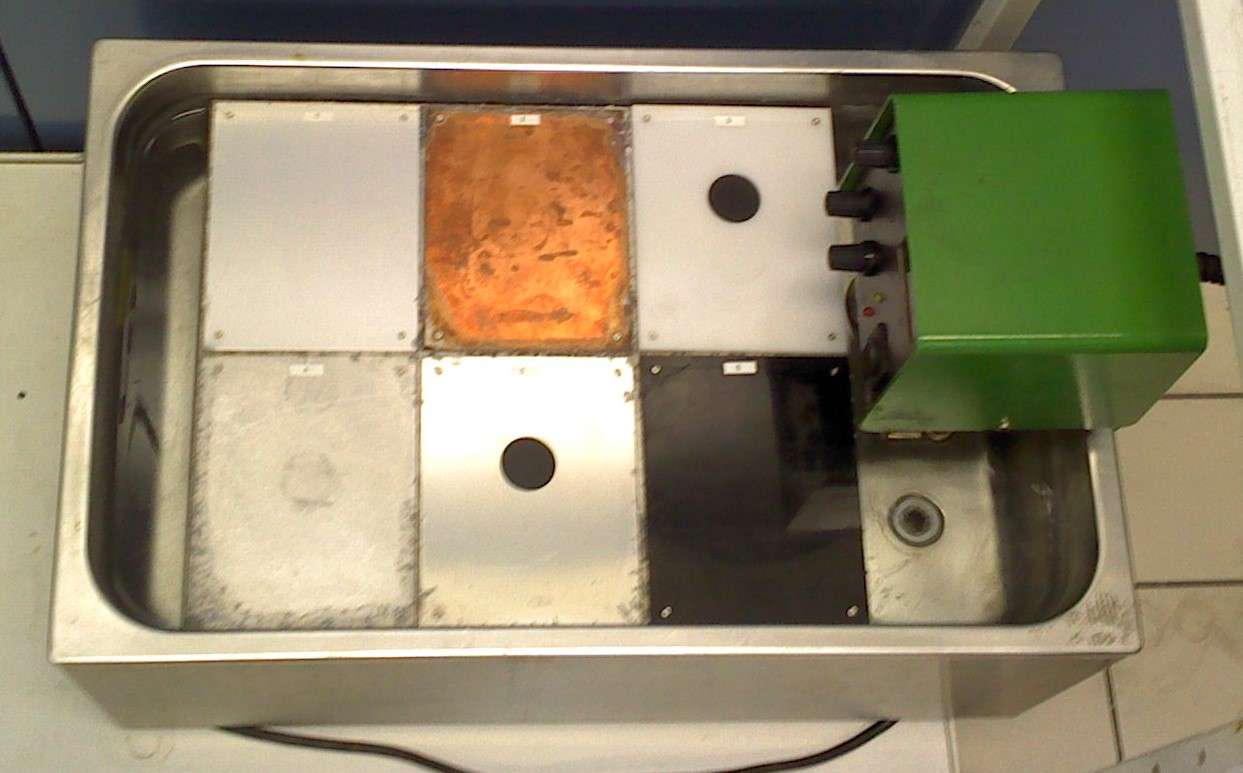
\includegraphics[width=0.5\textwidth]{../FLIR_100/FLIR2240.jpg}
		\caption{Versuchsaufbau Wärmebildkamera: Die unterschiedlichen Probenplatten wurden im selben Wärmebad mit \SI{60,0}{\celsius} temperiert.}
		\label{fig:VersuchsaufbauWBK}
\end{figure}

\begin{figure}[H]
		\centering
		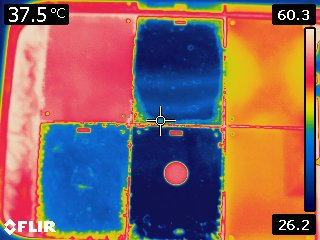
\includegraphics[width=0.4\textwidth]{../FLIR_100/FLIR2241.jpg}
		\caption{Foto der Wärmebildkamera über alle Probenplatten bei gleicher Temperatur.}
		\label{fig:FotoWBK}
\end{figure}

\begin{figure}[H]
		\centering
		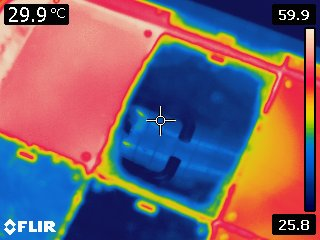
\includegraphics[width=0.4\textwidth]{../FLIR_100/FLIR2249.jpg}
		\caption[Ermitteltes Wärmekamerafoto mit Deckenbeleuchtung als Störfaktor]{Ermitteltes Wärmekamerafoto mit Deckenbeleuchtung als Störfaktor.}
		\label{fig:WBKHand}
\end{figure}

\begin{figure}[H]
		\centering
		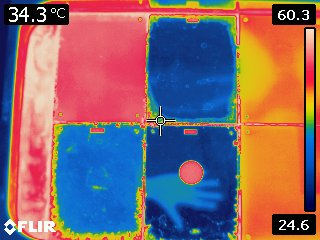
\includegraphics[width=0.4\textwidth]{../FLIR_100/FLIR2243.jpg}
		\caption[Ermitteltes Wärmekamerafoto mit Hand als Störfaktor]{Ermitteltes Wärmekamerafoto mit Hand als Störfaktor.}
		\label{fig:WBKDecke}
\end{figure}
